\DailyTitle{6352 Log (November 9, 2010)}

\DailySection{Goals}

\begin{enumerate}
\item 
\end{enumerate}

\DailySection{Summary List}

\begin{enumerate}
\item Flag validation.  Some residual remains.
\item Started running on HI data run 150431, \texttt{HIAllPhysics} stream.
\item Trying out reverse fit.  Doesn't work well.  Signal spread too much, and can go negative (fit better to reversed shape....)
\end{enumerate}

\DailySection{Flag validation}

Debugged a bit on flag setter.  Some points:

\begin{enumerate}
\item ``TS4 / Slope > limit'' is not the same as ``TS4 > limit * slope''.  There could be a sign problem when TS4 is negative.
We would like to cut this kind of pulse out (TS4 < 0) in any case, so..... maybe a protection system could help.
\item Towers (-1, 36, 1), (-5, 36, 1) and (-9, 36, 1) are inconsistent between flagger and offline fit across all noise types.
The source doesn't look simple to find out, though it would be useful to double-check what is going on here.
Also observed are some small energy pulses with apparent large charge in TS5.  This is also something to understand.
\item All other channels are consistent.
\end{enumerate}

\DailySection{First look at HI run 150431}

Keep all events after lumisection 151, according to the twiki page \url{https://twiki.cern.ch/twiki/bin/view/CMS/HIData2010RunInformation}.
See figures \ref{Figure_6352_FailLinear_Comparison}, \ref{Figure_6352_FailLinear_Geometry}, \ref{Figure_6352_FailRMS8Max_Comparison},
\ref{Figure_6352_FailRMS8Max_Geometry} and \ref{Figure_6352_FailSlopes_Geometry} for more information on pulses failing each condition.
Overall it looks like the ``noise purity'' is higher in this run compared to proton runs.  Flat noise is roughly the same geometrically
The distribution of different discriminants are shown in figure \ref{Figure_6352_Discriminants} for reference.
Noise distribution is pretty different.... the late-dropping ones are worth investigating.
HBHE MET distribution before and after cleaning is shown in figure \ref{Figure_6352_HBHEMET}.

ps. the ``signal'' here is partial statistics on run 147454 and 147754, after JP cleaning.  The HI run is also partial statistics, no selection applied.  Noise runs include 147454, 147754, 148058.

\begin{figure}
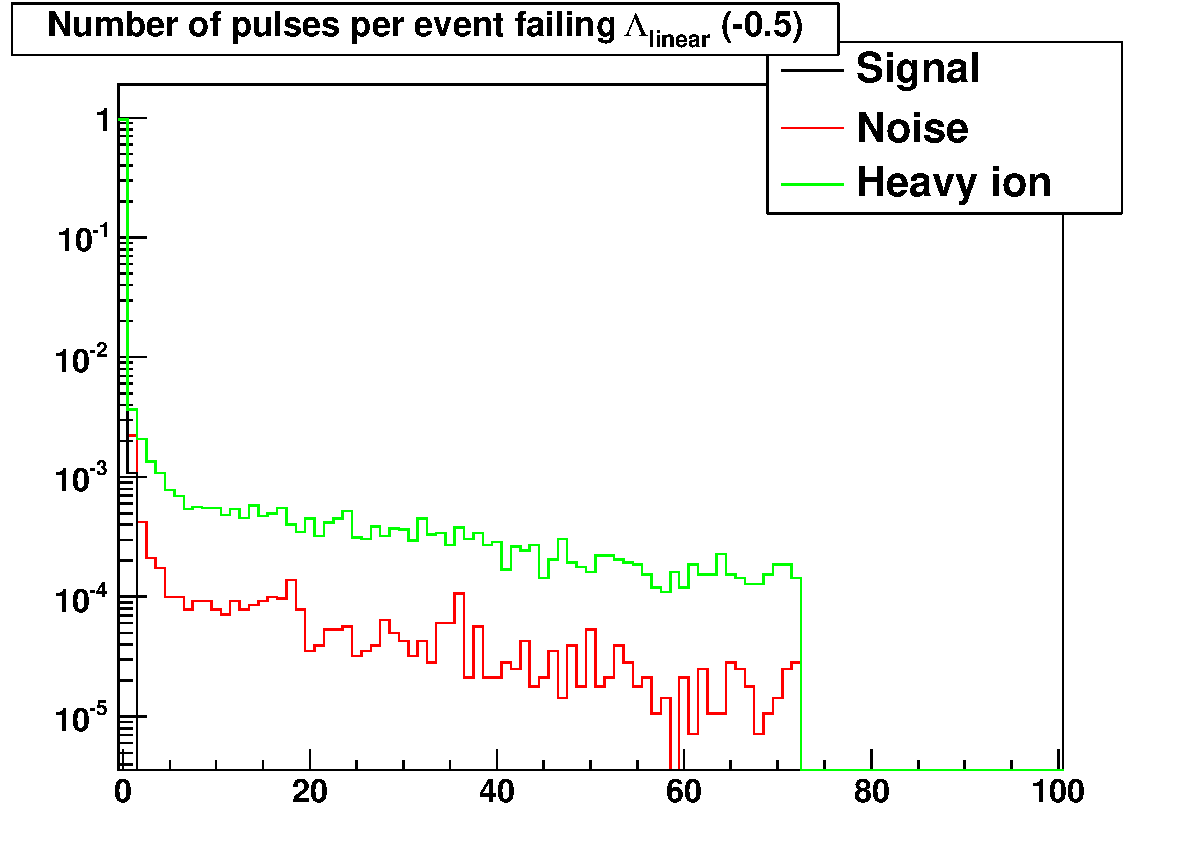
\includegraphics[width=120mm]{DailyLog/6352/6352_Comparison20_Comparison_HFailLambdaLinearCount}
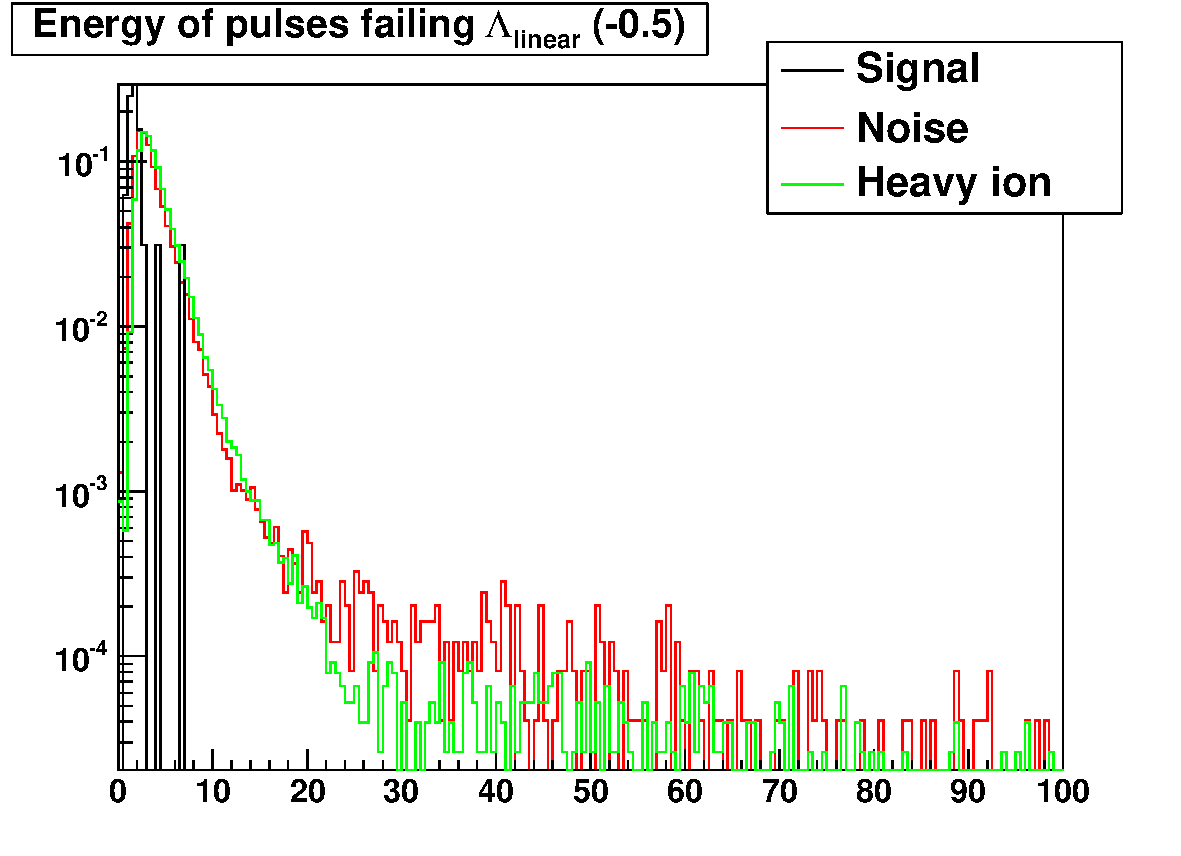
\includegraphics[width=120mm]{DailyLog/6352/6352_Comparison20_Comparison_HFailLambdaLinearEnergy}
\caption{Pulses failing linear discriminant}
\label{Figure_6352_FailLinear_Comparison}
\end{figure}

\begin{figure}
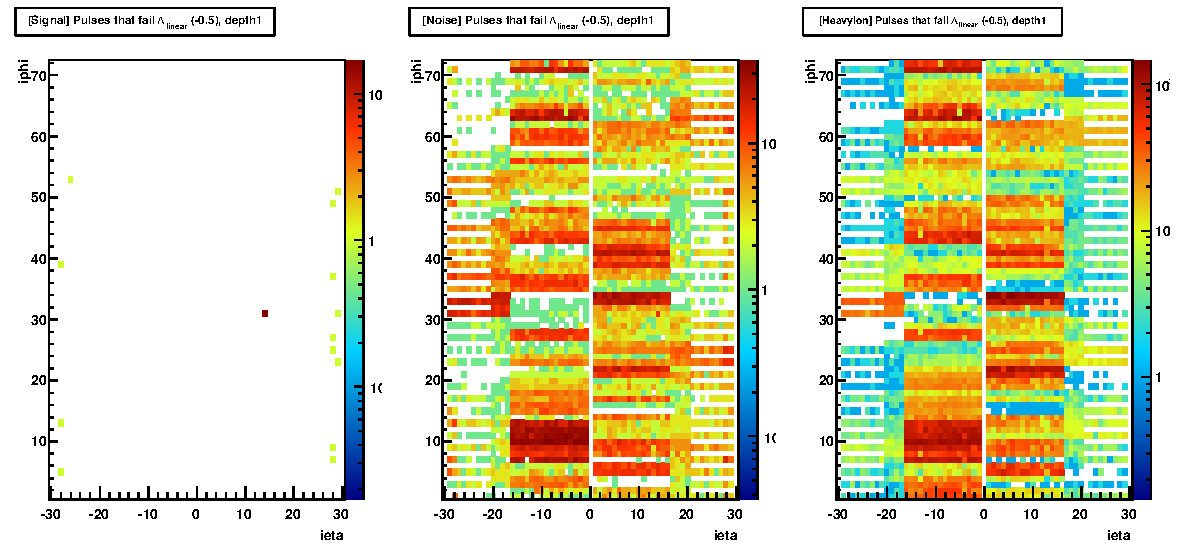
\includegraphics[width=120mm]{DailyLog/6352/6352_Comparison20_Comparison_HFailLambdaLinearIEtaIPhiDepth1}
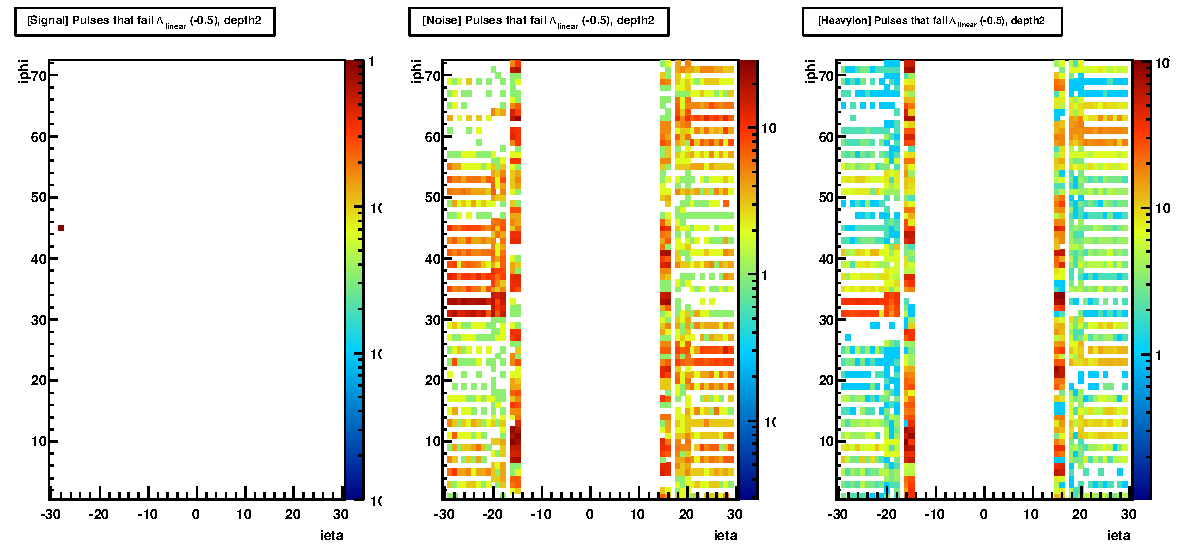
\includegraphics[width=120mm]{DailyLog/6352/6352_Comparison20_Comparison_HFailLambdaLinearIEtaIPhiDepth2}
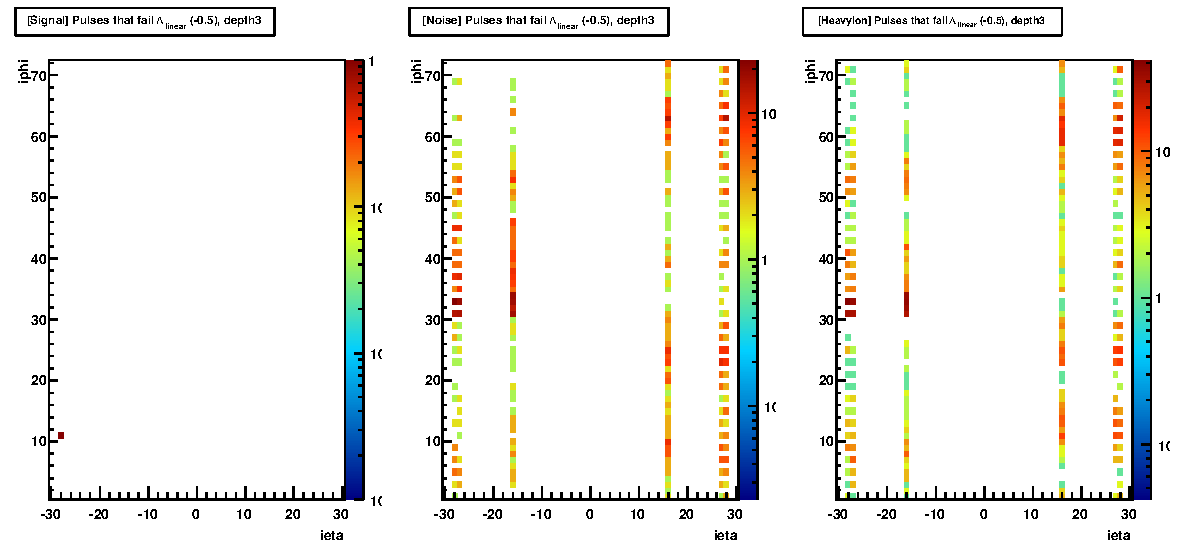
\includegraphics[width=120mm]{DailyLog/6352/6352_Comparison20_Comparison_HFailLambdaLinearIEtaIPhiDepth3}
\caption{Pulses failing linear discriminant}
\label{Figure_6352_FailLinear_Geometry}
\end{figure}

\begin{figure}
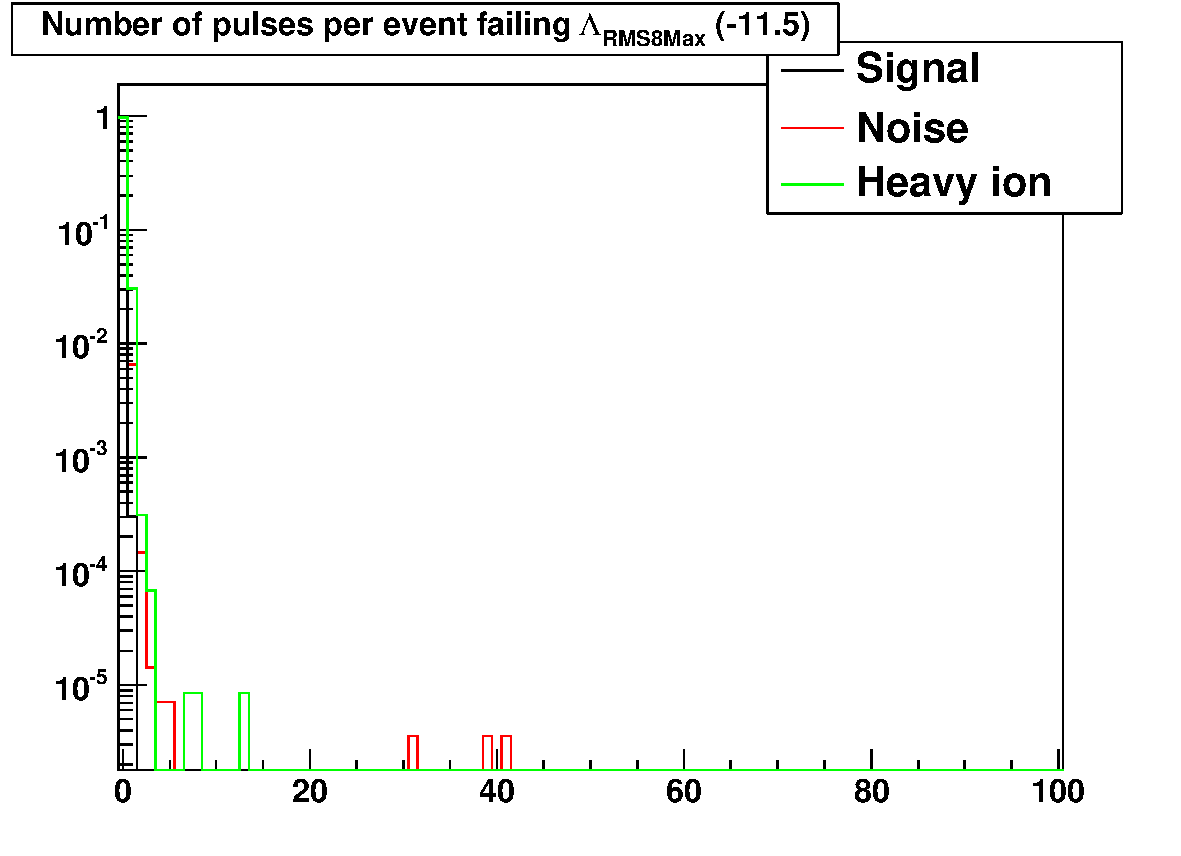
\includegraphics[width=120mm]{DailyLog/6352/6352_Comparison20_Comparison_HFailLambdaRMS8MaxCount}
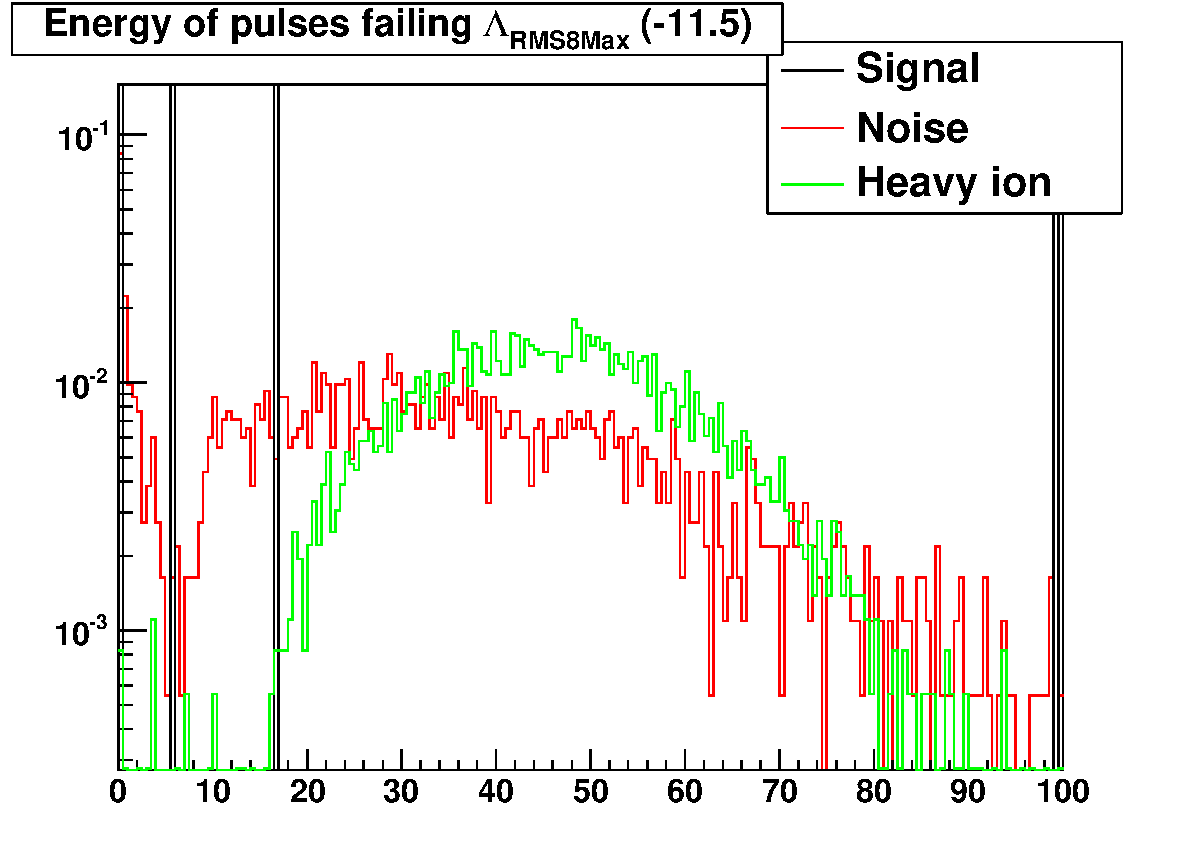
\includegraphics[width=120mm]{DailyLog/6352/6352_Comparison20_Comparison_HFailLambdaRMS8MaxEnergy}
\caption{Pulses failing RMS8/Max discriminant}
\label{Figure_6352_FailRMS8Max_Comparison}
\end{figure}

\begin{figure}
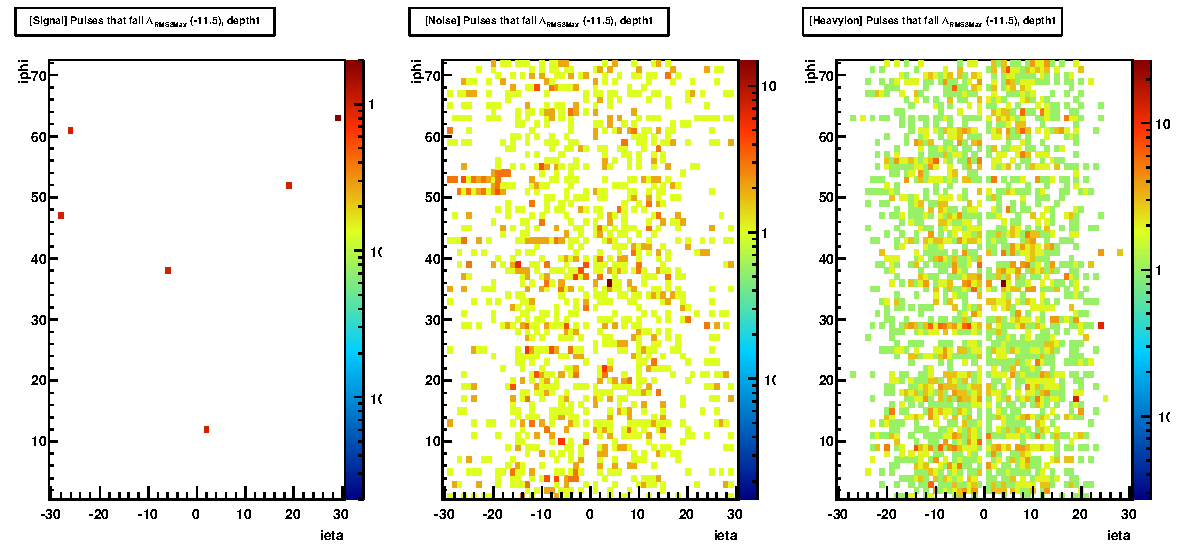
\includegraphics[width=120mm]{DailyLog/6352/6352_Comparison20_Comparison_HFailLambdaRMS8MaxIEtaIPhiDepth1}
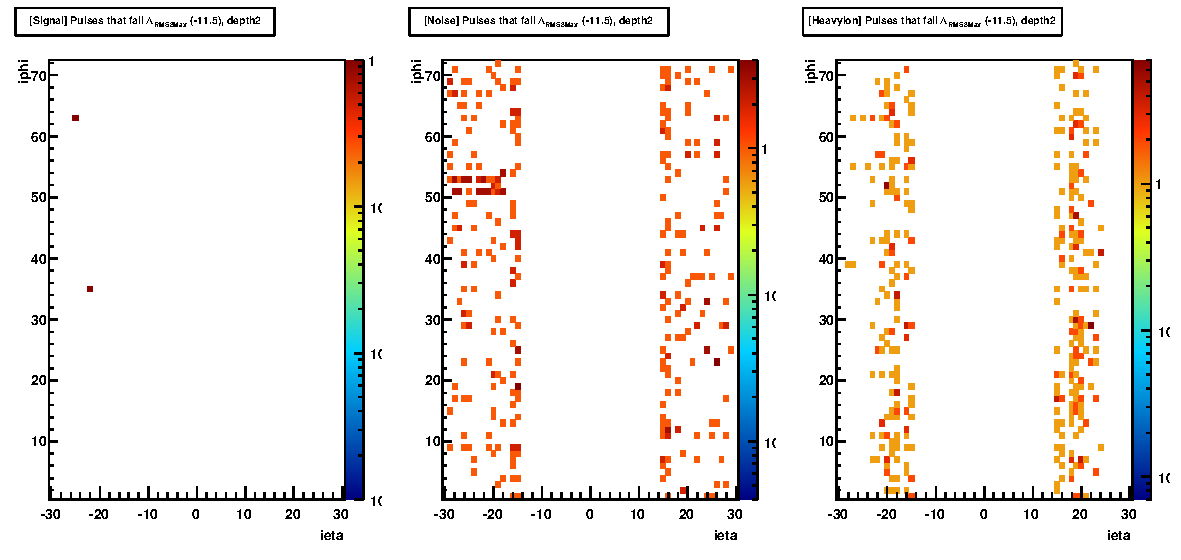
\includegraphics[width=120mm]{DailyLog/6352/6352_Comparison20_Comparison_HFailLambdaRMS8MaxIEtaIPhiDepth2}
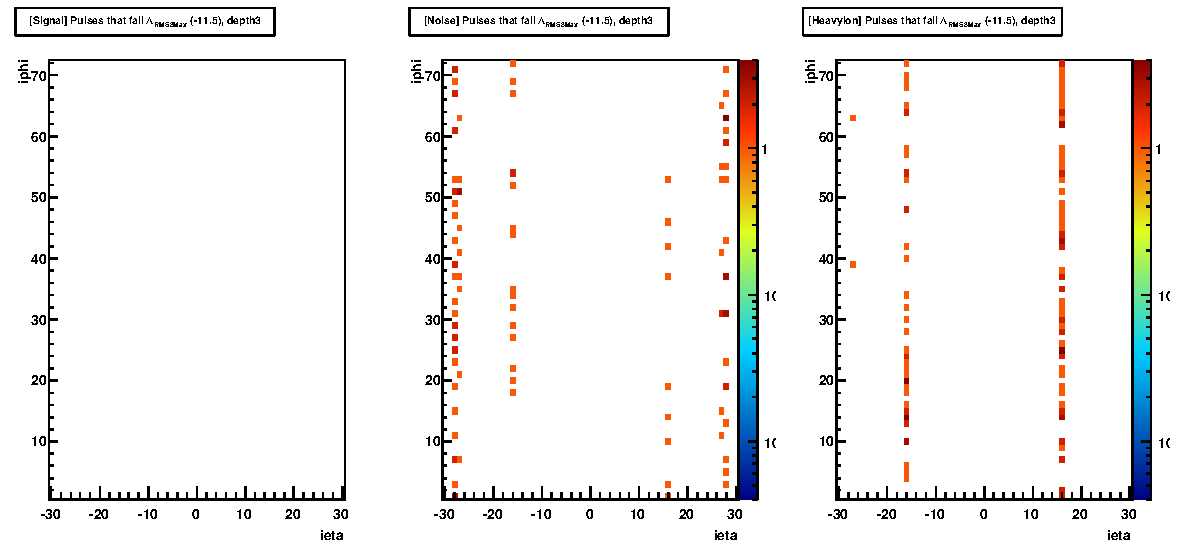
\includegraphics[width=120mm]{DailyLog/6352/6352_Comparison20_Comparison_HFailLambdaRMS8MaxIEtaIPhiDepth3}
\caption{Pulses failing RMS8/Max discriminant}
\label{Figure_6352_FailRMS8Max_Geometry}
\end{figure}

\begin{figure}
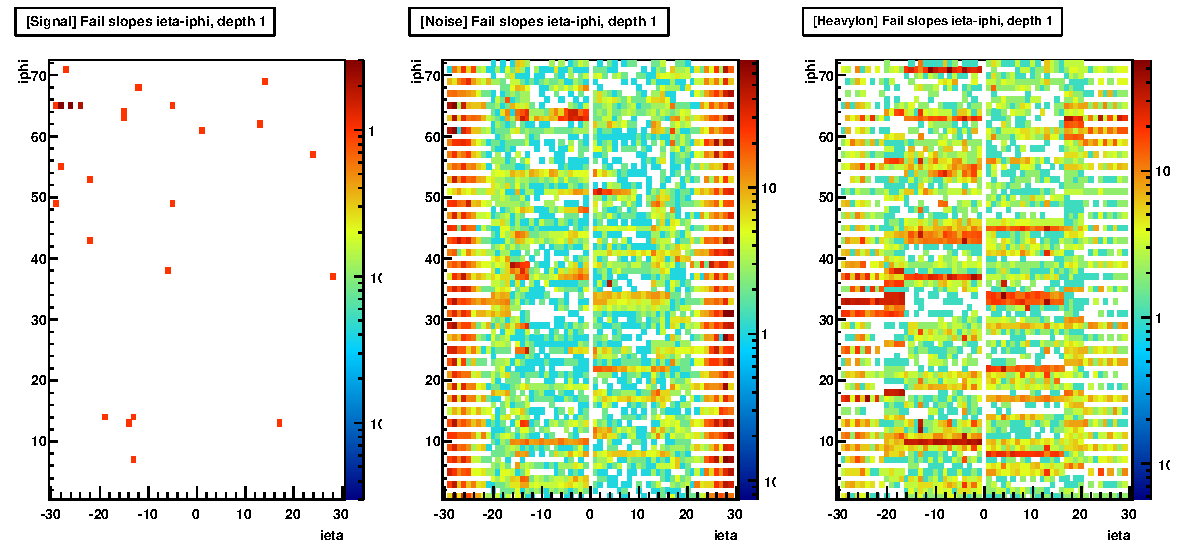
\includegraphics[width=120mm]{DailyLog/6352/6352_Comparison20_Comparison_HFailSlopesIEtaIPhiDepth1}
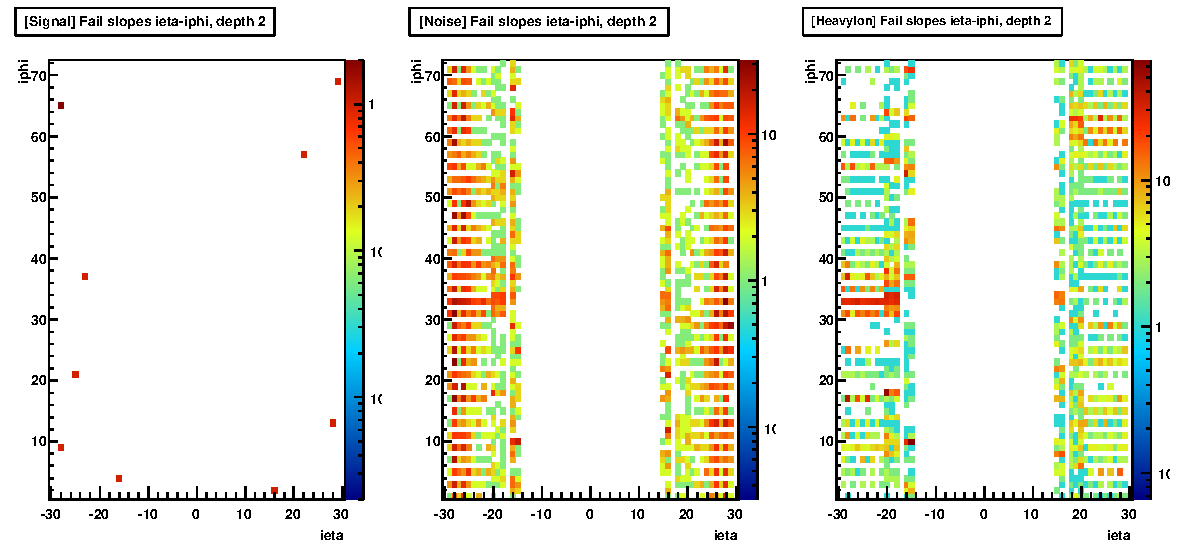
\includegraphics[width=120mm]{DailyLog/6352/6352_Comparison20_Comparison_HFailSlopesIEtaIPhiDepth2}
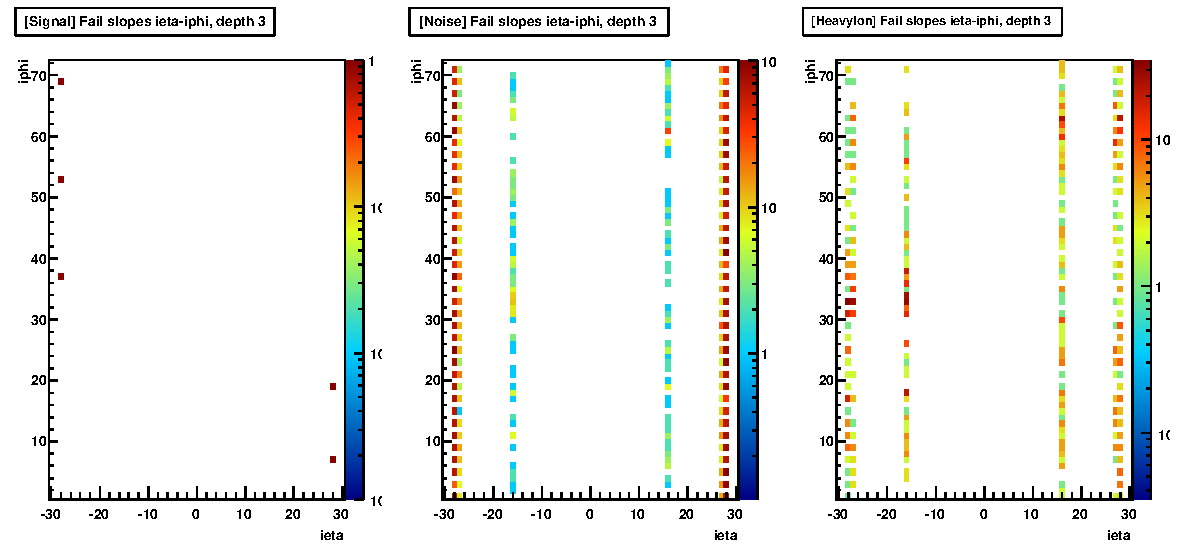
\includegraphics[width=120mm]{DailyLog/6352/6352_Comparison20_Comparison_HFailSlopesIEtaIPhiDepth3}
\caption{Pulses failing triangle fit slope}
\label{Figure_6352_FailSlopes_Geometry}
\end{figure}

\begin{figure}
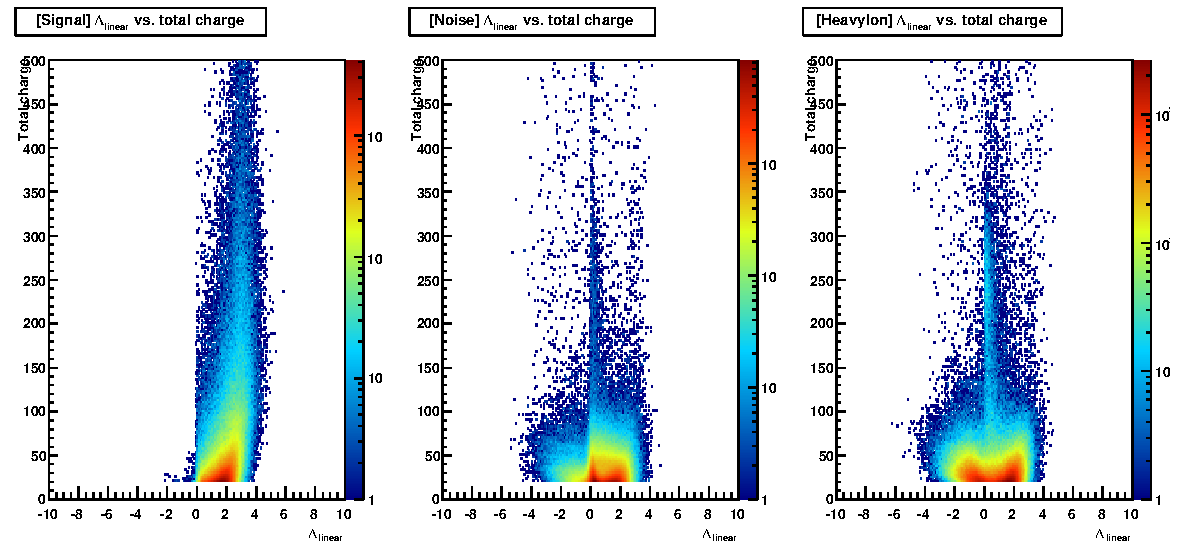
\includegraphics[width=120mm]{DailyLog/6352/6352_Comparison20_Comparison_HLambdaLinearVsTotalCharge}
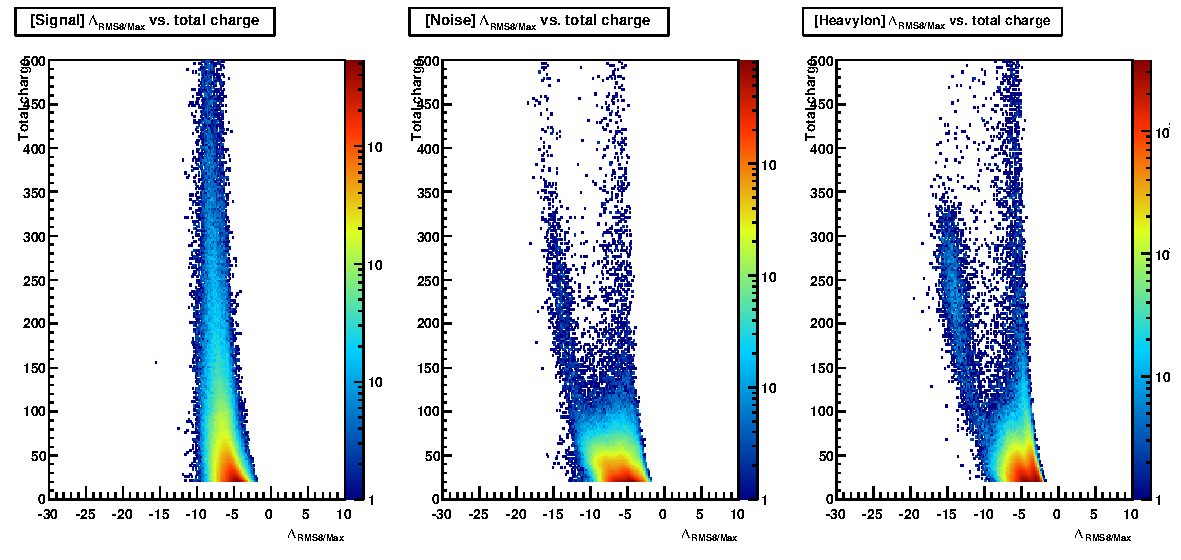
\includegraphics[width=120mm]{DailyLog/6352/6352_Comparison20_Comparison_HLambdaRMS8MaxVsTotalCharge}
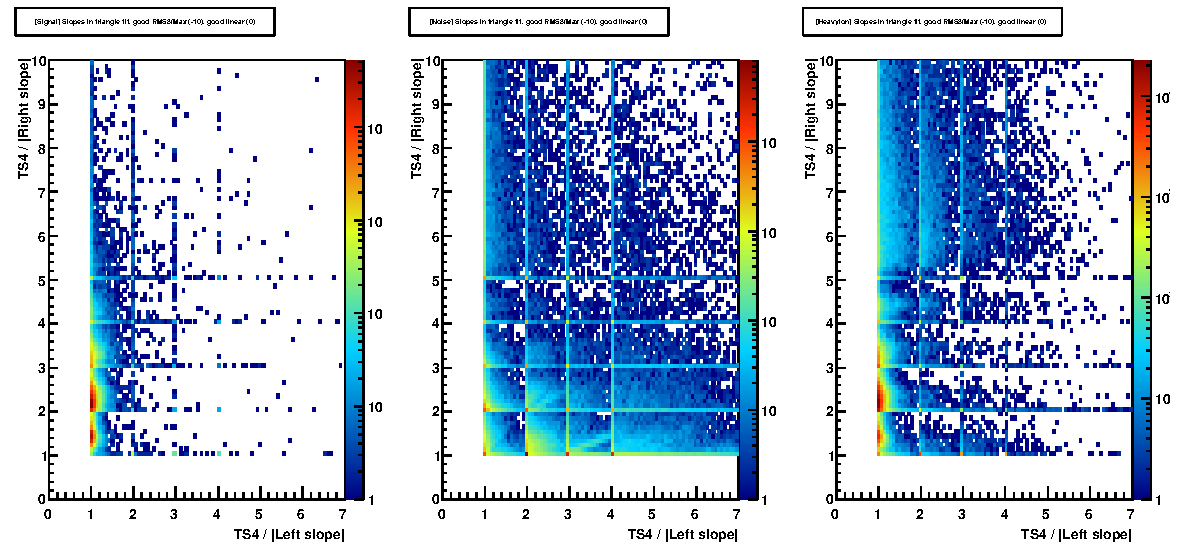
\includegraphics[width=120mm]{DailyLog/6352/6352_Comparison20_Comparison_HTriangleFitTS4OverSlopesGoodLinearGoodRMS8Max}
\caption{Distribution of main discriminants}
\label{Figure_6352_Discriminants}
\end{figure}

\begin{figure}
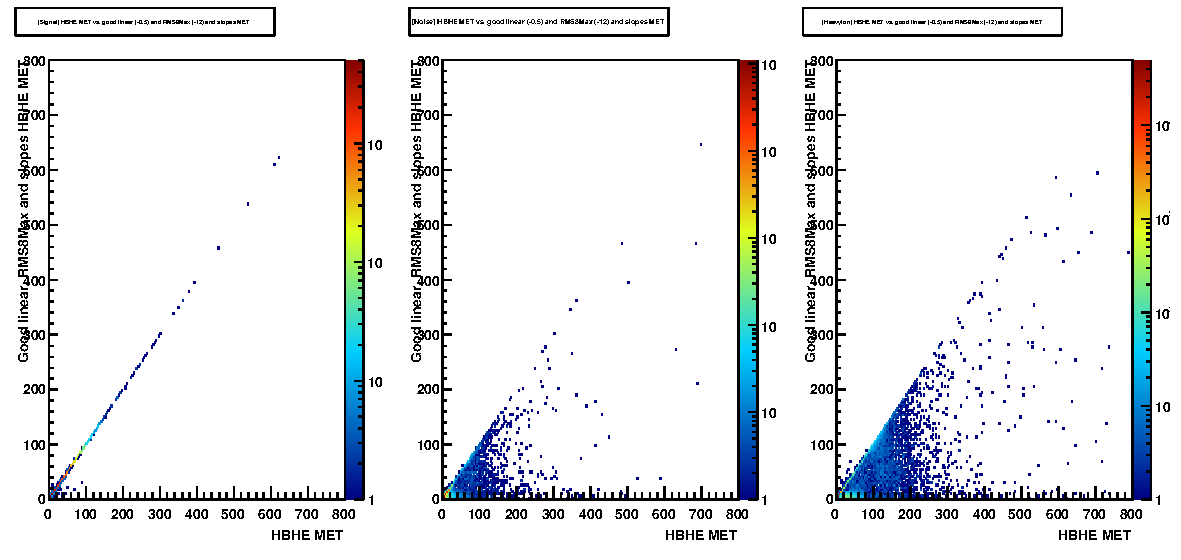
\includegraphics[width=120mm]{DailyLog/6352/6352_Comparison20_Comparison_HHBHEMETVsGoodLinearRMS8MaxSlopesHBHEMET}
\caption{HBHE MET distributions}
\label{Figure_6352_HBHEMET}
\end{figure}

\DailySection{TS3 investigation}

Time slice 3 itself cannot be used, but TS3 divided by total charge can be used to cut out a few percent of noise after round 1.
It's too far from the fitting framework, it might be better to find a fit that includes this behavior.


\DailySection{Reflection}

\DailySection{Goals for next work day}

\begin{enumerate}
\item Eat lunch
\item Eat dinner
\item Find the red herring
\end{enumerate}


